\section{Raytracing-related Objects}\label{sec:raytracing-objects}

In this section we will take a closer look at all the objects related to ray tracing and our abstractions of them.

\subsection{Acceleration Structures}

We are going to start with the acceleration structures. Acceleration structures are data structures used by the implementation to efficiently manage scene geometry as it is traversed during a ray tracing query~\parencite{vulkan-spec-as}. The acceleration structure has two levels:

\begin{itemize}
    \item \textbf{Bottom Level Acceleration Structure (BLAS)}
    
    The lower level, the bottom-level acceleration structure, contains the triangles or axis-aligned bounding boxes (AABBs) of custom geometry that make up the scene~\parencite{raytracing-in-vulkan}. The BLAS usually corresponds to a mesh that is used in a scene.

    \item \textbf{Top Level Acceleration Structure (TLAS)}
    
    The upper level, the top-level acceleration structure, contains references to a set of bottom-level acceleration structures, each reference including shading and transform information for that reference~\parencite{raytracing-in-vulkan}. The TLAS represents a scene filled with objects, each of which can have a different transformation and a mesh.
\end{itemize}

The relationship between TLAS and BLAS can be seen in \autoref{fig:acceleration-structure}.

\begin{figure}[H]
    \centering
    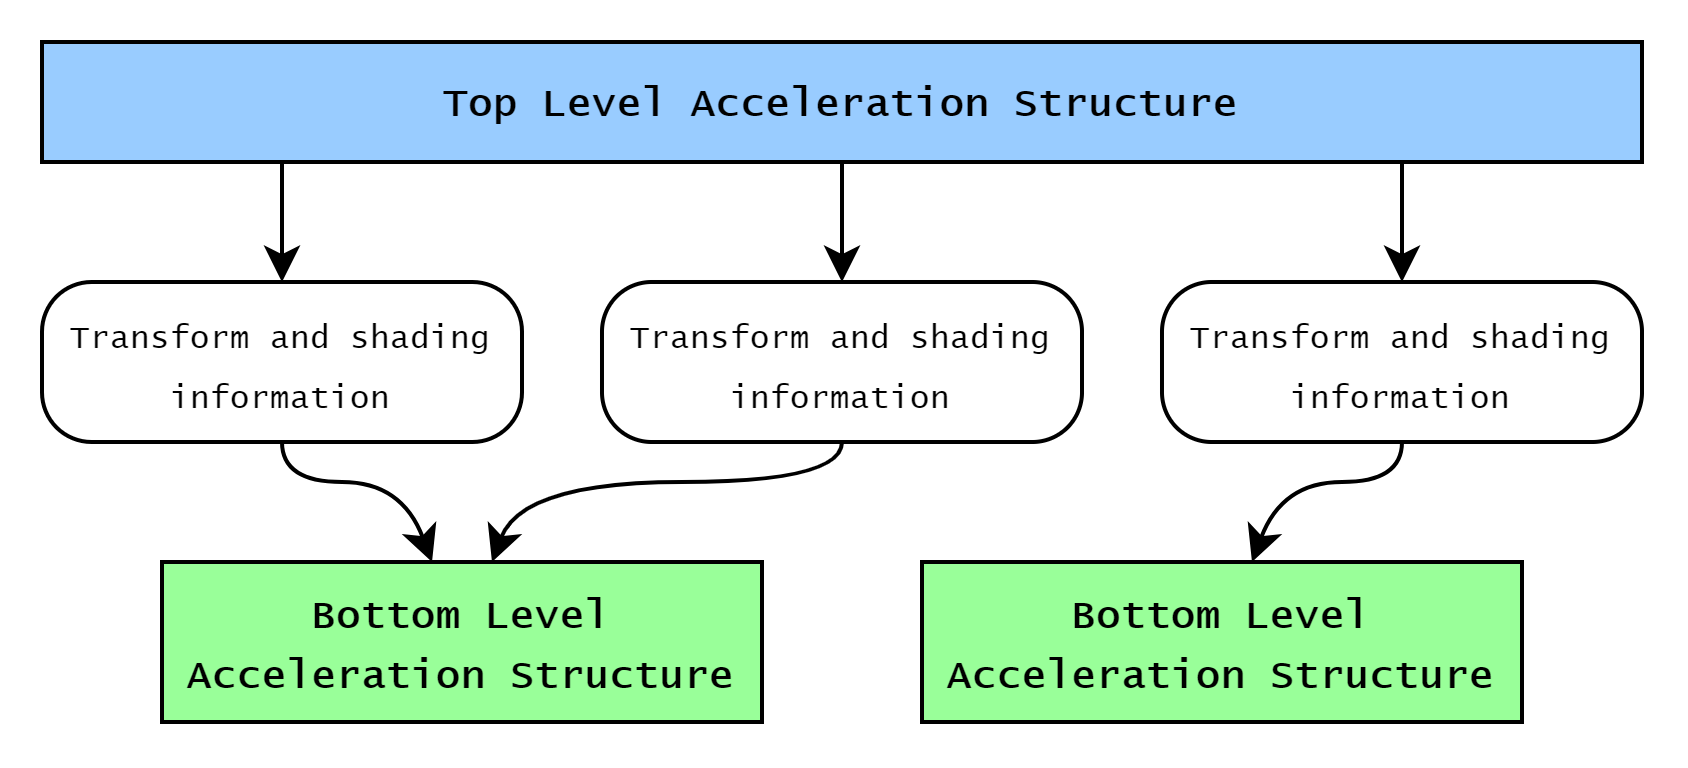
\includegraphics[width=0.8\textwidth]{figures/acceleration_structure.png}
    \caption{Acceleration structure}
    \label{fig:acceleration-structure}
\end{figure}

Vulkan represents both types using the \code{VkAccelerationStructureKHR} handle. This handle only contains some metadata; the actual data of the acceleration structure (e.g., the BVH) is stored in a \code{VkBuffer}. Before building an acceleration structure, we need to reference the data used for building in a \code{VkAccelerationStructureGeometryKHR}. For a BLAS, this is typically a list of triangles (other primitives are also possible), and for a TLAS, it is a list of instances containing transformation and shading information, as well as a handle to a BLAS. Once the \code{VkAccelerationStructureGeometryKHR} is prepared, we can query \code{VkAccelerationStructureBuildSizesInfoKHR}, which contains \code{accelerationStructureSize} (the buffer size for the acceleration structure) and \code{updateScratchSize} and \code{buildScratchSize} (the sizes of temporary scratch buffers used during building or updating). Finally, we can build the acceleration structure using \code{vkCmdBuildAccelerationStructuresKHR}.

We encapsulate a BLAS and TLAS in the classes \code{Blas} and \code{Tlas}, respectively. They both have the following member variables:

\begin{itemize}
    \item \code{blas}/\code{tlas}: The \code{Handle<VkAccelerationStructureKHR>}.
    \item \code{buffer}: The buffer that stores the acceleration structure data.
    \item \code{build\_scratch\_buffer}: The scratch buffer used during building.
    \item \code{update\_scratch\_buffer}: The scratch buffer used during updating/refitting.
\end{itemize}

These classes also have a builder (see \autoref{subsec:builder-pattern} and \autoref{subsec:basic-vulkan-object}), which expects a list of \code{BlasGeometry}s when building a \code{Blas} and a list of \code{TlasInstance}s when building a \code{Tlas}. A \code{BlasGeometry} describes the vertex buffer and optional index buffer used for a triangle mesh, while a \code{TlasInstance} stores a reference to a BLAS in a \code{ptr::Shared<Blas>} together with a transformation. The builder has a \code{dynamic} property, which must be set to \code{true} if the acceleration structure will be refitted later. It also has a \code{fast\_build} property, which, if set to \code{true}, will prefer a fast build over fast tracing by setting the flag \code{PREFER\_FAST\_BUILD} instead of \code{PREFER\_FAST\_TRACE}.

There are two ways to update an acceleration structure:

\begin{itemize}
    \item \code{rebuild}
    
    Recreates the BVH from scratch. It performs the same steps as the builder's \code{build} function, but uses the already created handle and buffers without creating them again.

    \item \code{refit}

    Adjusts only the bounds of the AABBs in the existing BVH according to new vertex positions, which is faster than rebuilding from scratch but may result in a suboptimal BVH, which can increase ray tracing time.

\end{itemize}

\subsection{Raytracing Pipeline}

To issue ray tracing commands, we need a ray tracing pipeline. \autoref{fig:raytracing-pipeline} shows a flow chart of the pipeline.

\begin{figure}[H]
    \centering
    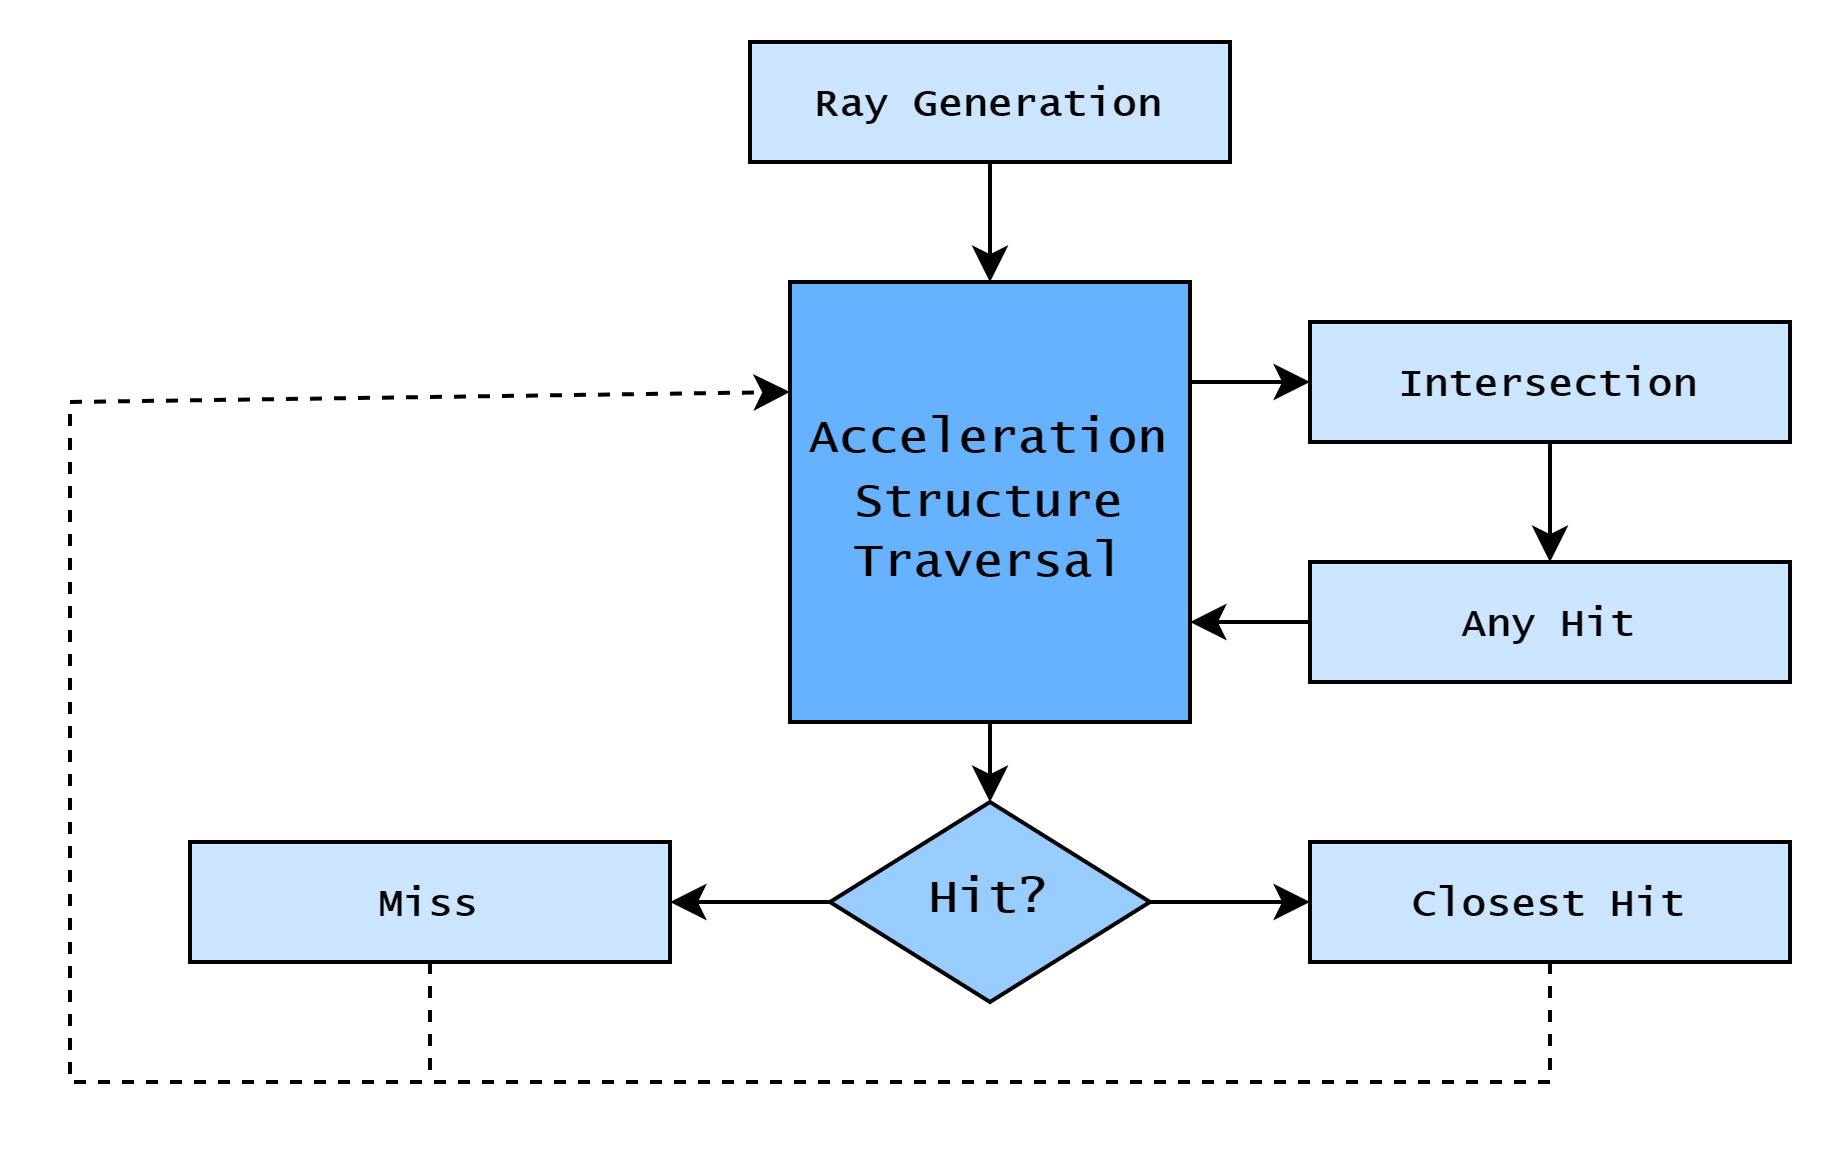
\includegraphics[width=0.8\textwidth]{figures/raytracing_pipeline.png}
    \caption{Ray tracing pipeline}
    \label{fig:raytracing-pipeline}
\end{figure}

A Vulkan raytracing pipeline organizes shaders into shader groups. In our application, we use two types:

\begin{itemize}
    \item \textbf{General Shader Group}
    
    A general shader group contains a single general shader that can be called independently of any ray/triangle intersection. This type is used in the ray generation and miss stages.

    \item \textbf{Triangle Hit Shader Group}
    
    A triangle hit shader group contains an any-hit shader and a closest-hit shader, executed when a ray intersects a triangle. The any-hit shader runs for every intersection along the ray, while the closest-hit shader runs only for the first intersection.

\end{itemize}

The class \code{ShaderGroup} implements shader groups in our application. Each \code{ShaderGroup} has a unique identifier accessible via the function \code{id}. It stores either a \code{ShaderGroupGeneral} or a \code{ShaderGroupHit} struct in a \code{std::variant}. \code{ShaderGroupGeneral} contains the \code{general} shader, while \code{ShaderGroupHit} contains \code{closest\_hit} and \code{any\_hit} shaders.

The raytracing pipeline is encapsulated in the class \code{RtxPipeline}, which is created from a list of \code{ShaderGroup}s. The \code{ShaderGroup} objects are only descriptions; the pipeline allocates the actual shader groups and stores a list of shader group handles. \code{RtxPipeline} also maintains a map from each \code{ShaderGroup} ID to the index of the shader group handle array for easy access.

The pipeline also needs a pipeline layout, given by a \code{PipelineLayout} object, and a maximum recursion depth (\code{max\_ray\_recursion\_depth}) for rays.

\subsection{Shader Binding Table}

Once the ray tracing pipeline is ready we need to create a shader binding table (SBT), which selects the correct shader group in every stage of the raytracing pipeline.

\begin{figure}[H]
    \centering
    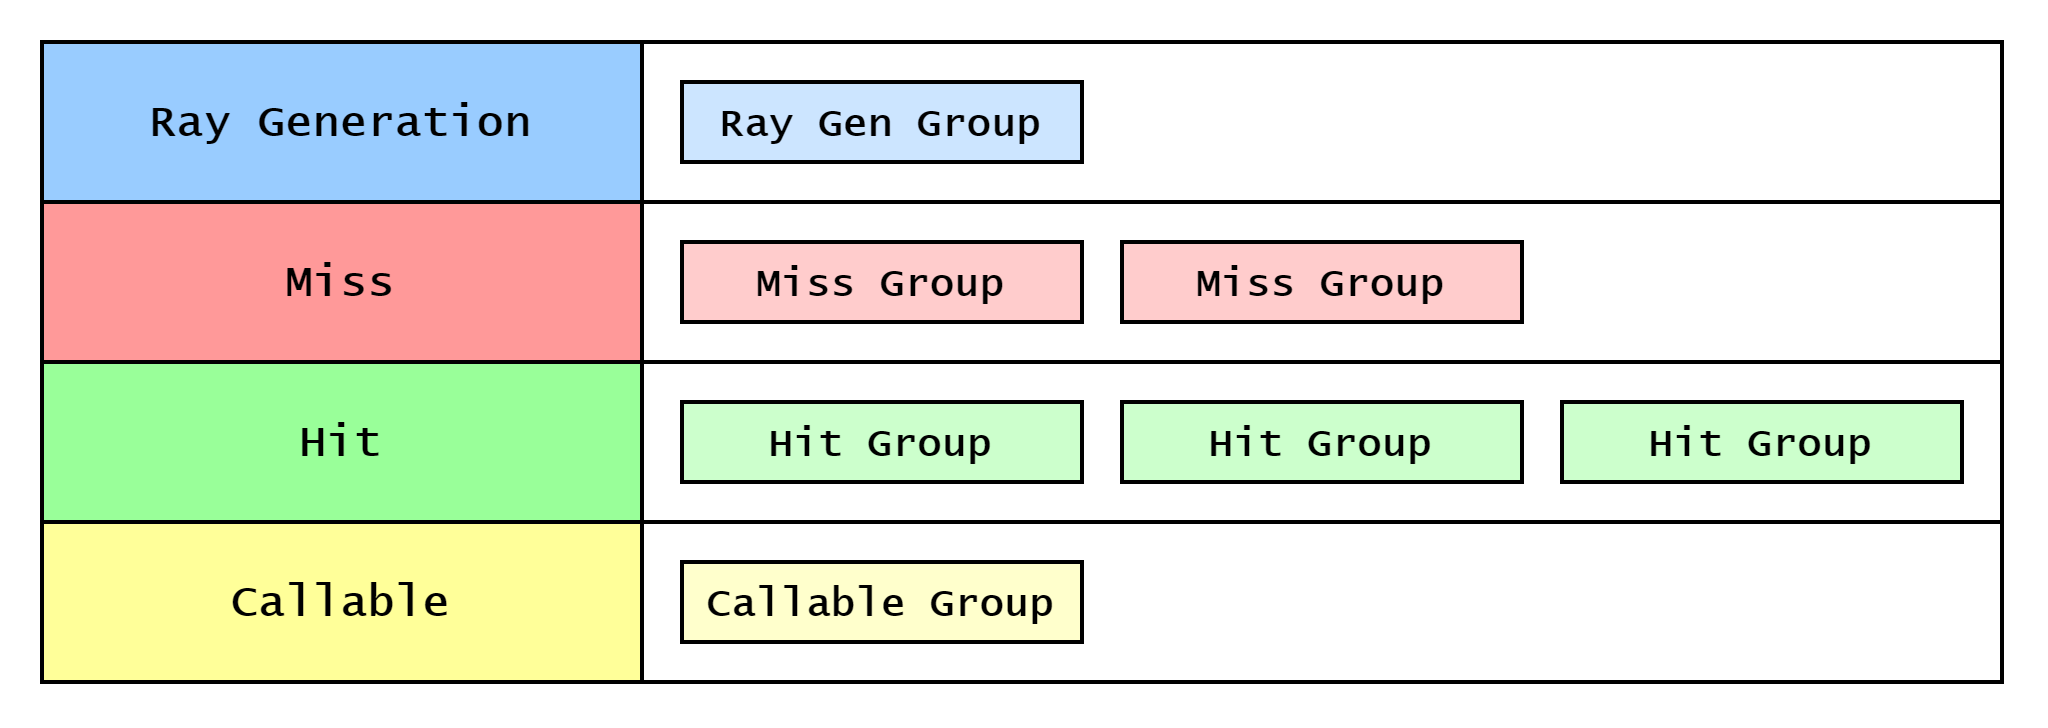
\includegraphics[width=0.9\textwidth]{figures/sbt.png}
    \caption{Shader binding table}
    \label{fig:sbt}
\end{figure}

As seen in \autoref{fig:sbt}, the SBT has four rows:

\begin{itemize}
\item \textbf{Ray Generation}: Shader group used for ray generation.
\item \textbf{Miss}: Shader groups used when a ray misses.
\item \textbf{Hit}: Shader groups used when a ray intersects at least one object.
\item \textbf{Callable}: Arbitrary shaders callable by other shaders, not tied to a specific ray traversal event (not used in our application).
\end{itemize}

The SBT is stored in a \code{VkBuffer}. A \code{VkStridedDeviceAddressRegionKHR}, which references a buffer region and specifies the stride between elements, represents a row in the SBT.

When casting a ray with \code{traceRayEXT}, we can specify a miss offset and a hit offset, indicating which shader group to use. Each TLAS instance can also define an additional offset for the hit shader group, added to the previous offset.

The SBT is implemented in the \code{SBT} class. Since the SBT strongly depends on the raytracing pipeline, it does not use a builder. Instead, it is built using the \code{build\_sbt} function in \code{RtxPipeline}, with a \code{SBTInfo} struct as a parameter. \code{SBTInfo} contains:

\begin{itemize}
    \item \code{ray\_gen\_group}: The \code{ShaderGroup} used for ray generation.
    \item \code{miss\_groups}: A list of \code{ShaderGroup}s, which can be used when a ray misses.
    \item \code{hit\_groups}: A list of \code{ShaderGroup}s, which can be used when a ray hits.
\end{itemize}

The \code{ShaderGroup}s in \code{SBTInfo} must be a subset of the shader groups used to create the pipeline. When building the SBT, we first retrieve the array of shader group handles using \code{vkGetRayTracingShaderGroupHandlesKHR}. Using the ID-to-index map, we get the handle for each shader group and store them in the SBT buffer: ray generation first, followed by miss shaders, then hit shaders. Finally, the \code{VkStridedDeviceAddressRegionKHR} is set for each row, and the SBT is ready for use in \code{vkCmdTraceRaysKHR}.

The code sample in \autoref{fig:pipeline-and-sbt-creation} shows the creation of a ray tracing pipeline and SBT:

\begin{figure}[H]
\begin{lstlisting}[language=C++]
// creating shader groups from shaders
ShaderGroup ray_gen_group = ShaderGroup::create_general(ray_gen_shader);
ShaderGroup miss_group = ShaderGroup::create_general(miss_shader);
...
ShaderGroup hit_group = ShaderGroup::create_hit_closest(closest_hit_shader);
...

//creating the ray tracing pipeline
RtxPipeline pipeline = RtxPipelineBuilder()
    .add_shader_group(ray_gen_group)
    .add_shader_group(miss_group)
    .add_shader_group(hit_group)
        ...
    .layout(pipeline_layout)
    .max_ray_recursion_depth(1)
    .build();

//createing the SBT
SBT sbt = pipeline.build_sbt(SBTInfo()
    .ray_gen_group(ray_gen_group)     // ray gen row
    .miss_groups({ miss_group, ... }) // miss row
    .hit_groups({ hit_group, ... })); // hit row


\end{lstlisting}
\caption{Sample-code to create ray tracing pipeline and SBT}
\label{fig:pipeline-and-sbt-creation}
\end{figure}

\pagebreak